% -------------------------------------------------- %
% >> ------------------ 宏定义 ------------------ << %

% 本文的特殊宏定义

% 通用宏定义
    \def\N{\mathbb{N}}
    \def\F{\mathbb{F}}
    \def\Z{\mathbb{Z}}
    \def\Q{\mathbb{Q}}
    \def\R{\mathbb{R}}
    \def\C{\mathbb{C}}
    \def\T{\mathbb{T}}
    \def\S{\mathbb{S}}
    \def\A{\mathbb{A}}
    \def\I{\mathscr{I}}
    \def\d{\mathrm{d}}
    \def\p{\partial}
    \def\Re{\,\mathrm{Re}\,}
    \def\Im{\,\mathrm{Im}\,}


% >> ------------------ 宏定义 ------------------ << %
% -------------------------------------------------- %


% ------------------------------------------------------------- %
% >> ------------------ 文章宏包及相关设置 ------------------ << %

\documentclass[a4paper]{article}  % 设定文章类型与编码格式

\usepackage[utf8]{inputenc}  
\usepackage[T1]{fontenc}  % 设置文档的字体编码为 T1 以支持更多的字符
\usepackage[english]{babel} % 如果你需要英文支持  
\usepackage{fancyhdr} % 用于页眉页脚  

% 导入基本宏包
    \usepackage[UTF8]{ctex}     % 设置文档为中文语言
        \usepackage{hyperref}  % 宏包:自动生成超链接 (此宏包与标题中的数学环境冲突)
    \hypersetup{
        colorlinks=true,    % false:边框链接 ; true:彩色链接
        citecolor={blue},    % 文献引用颜色
        linkcolor={blue},   % 目录 (我们在目录处单独设置),公式,图表,脚注等内部链接颜色
        urlcolor={magenta},    % 网页 URL 链接颜色,包括 \href 中的 text
        % cyan 浅蓝色 
        % magenta 洋红色
        % yellow 黄色
        % black 黑色
        % white 白色
        % red 红色
        % green 绿色
        % blue 蓝色
        % gray 灰色
        % darkgray 深灰色
        % lightgray 浅灰色
        % brown 棕色
        % lime 石灰色
        % olive 橄榄色
        % orange 橙色
        % pink 粉红色
        % purple 紫色
        % teal 蓝绿色
        % violet 紫罗兰色
    }
    % \usepackage{docmute}    % 宏包:子文件导入时自动去除导言区,用于主/子文件的写作方式,\include{./51单片机笔记}即可。注:启用此宏包会导致.tex文件capacity受限。
    \usepackage{amsmath}    % 宏包:数学公式
    \usepackage{mathrsfs}   % 宏包:提供更多数学符号
    \usepackage{amssymb}    % 宏包:提供更多数学符号
    \usepackage{pifont}     % 宏包:提供了特殊符号和字体
    \usepackage{extarrows}  % 宏包:更多箭头符号

%宏包:有色文本框(proof环境)及其设置
\usepackage[dvipsnames,svgnames]{xcolor}    %设置插入的文本框颜色
\usepackage[strict]{changepage}     % 提供一个 adjustwidth 环境
\usepackage{framed}     % 实现方框效果
    \definecolor{graybox_color}{rgb}{0.95,0.95,0.96} % 文本框颜色。修改此行中的 rgb 数值即可改变方框纹颜色,具体颜色的rgb数值可以在网站https://colordrop.io/ 中获得。(截止目前的尝试还没有成功过,感觉单位不一样)(找到喜欢的颜色,点击下方的小眼睛,找到rgb值,复制修改即可)
    \newenvironment{graybox}{%
    \def\FrameCommand{%
    \hspace{1pt}%
    {\color{gray}\small \vrule width 2pt}%
    {\color{graybox_color}\vrule width 4pt}%
    \colorbox{graybox_color}%
    }%
    \MakeFramed{\advance\hsize-\width\FrameRestore}%
    \noindent\hspace{-4.55pt}% disable indenting first paragraph
    \begin{adjustwidth}{}{7pt}%
    \vspace{2pt}\vspace{2pt}%
    }
    {%
    \vspace{2pt}\end{adjustwidth}\endMakeFramed%
    }


% 配置数学环境
    \usepackage{amsthm} % 宏包:数学环境配置
    % theorem-line 环境自定义
        \newtheoremstyle{MyLineTheoremStyle}% <name>
            {11pt}% <space above>
            {11pt}% <space below>
            {\kaishu}% <body font> 使用默认正文字体
            {}% <indent amount>
            {\bfseries}% <theorem head font> 设置标题项为加粗
            {:}% <punctuation after theorem head>
            {.5em}% <space after theorem head>
            {\textbf{#1}\thmnumber{#2}\ \ (\,\textbf{#3}\,)}% 设置标题内容顺序
        \theoremstyle{MyLineTheoremStyle} % 应用自定义的定理样式
        \newtheorem{LineTheorem}{Theorem.\,}
    % theorem-block 环境自定义
        \newtheoremstyle{MyBlockTheoremStyle}% <name>
            {11pt}% <space above>
            {11pt}% <space below>
            {\kaishu}% <body font> 使用默认正文字体
            {}% <indent amount>
            {\bfseries}% <theorem head font> 设置标题项为加粗
            {:\\ \indent}% <punctuation after theorem head>
            {.5em}% <space after theorem head>
            {\textbf{#1}\thmnumber{#2}\ \ (\,\textbf{#3}\,)}% 设置标题内容顺序
        \theoremstyle{MyBlockTheoremStyle} % 应用自定义的定理样式
        \newtheorem{BlockTheorem}[LineTheorem]{Theorem.\,} % 使用 LineTheorem 的计数器
    % definition 环境自定义
        \newtheoremstyle{MySubsubsectionStyle}% <name>
            {11pt}% <space above>
            {11pt}% <space below>
            {}% <body font> 使用默认正文字体
            {}% <indent amount>
            {\bfseries}% <theorem head font> 设置标题项为加粗
            {:\\ \indent}% <punctuation after theorem head>
            {0pt}% <space after theorem head>
            {\textbf{#3}}% 设置标题内容顺序
        \theoremstyle{MySubsubsectionStyle} % 应用自定义的定理样式
        \newtheorem{definition}{}

% table 支持
    \usepackage{booktabs}   % 宏包:三线表
    \usepackage{tabularray} % 宏包:表格排版
    \usepackage{longtable}  % 宏包:长表格

% figure 设置
    \usepackage{graphicx}  % 支持 jpg, png, eps, pdf 图片 
    \usepackage{svg}       % 支持 svg 图片
        \svgsetup{
            % 指向 inkscape.exe 的路径
            %inkscapeexe = C:/aa_MySame/inkscape/bin/inkscape.exe, 
            inkscapeexe = D:/aa_MyApps/inkscape/bin/inkscape.exe, 
            % 一定程度上修复导入后图片文字溢出几何图形的问题
            inkscapelatex = false                 
        }
    \usepackage[skip=0.6pt]{subcaption} % subfigure 子图支持
    \usepackage{caption}    % 图注、表注
        \captionsetup[figure]{name=图, skip=0.8pt}    % 图注名称为 '图', 并修改 skip 间距
        \captionsetup[table]{name=表, skip=0.8pt}
        \captionsetup{
            labelfont=bf, % 设置标签为粗体
            textfont=bf,  % 设置文本为粗体
            font=small  
        }
    \usepackage{float}     % 图表位置浮动设置 
    \usepackage{etoolbox} % 用于保证图注表注的数学字符为粗体
        \AtBeginEnvironment{figure}{\boldmath} % 图注中的数学字符为粗体
        \AtBeginEnvironment{table}{\boldmath}  % 表注中的数学字符为粗体
        \AtBeginEnvironment{tabular}{\unboldmath}   % 保证表格中的数学字符不受额外影响
% 列表设置
\usepackage{enumitem}   % 宏包:列表环境设置
    \setlist[enumerate]{
        label=(\arabic*) ,   % 设置序号样式为加粗的 (1) (2) (3)
        ref=\arabic*, % 如果需要引用列表项,这将决定引用格式(这里仍然使用数字)
        itemsep=0pt, parsep=0pt, topsep=0pt, partopsep=0pt, leftmargin=3.5em} 
    \setlist[itemize]{itemsep=0pt, parsep=0pt, topsep=0pt, partopsep=0pt, leftmargin=3.5em}
    \newlist{circledenum}{enumerate}{1} % 创建一个新的枚举环境  
    \setlist[circledenum,1]{  
        label=\protect\circled{\arabic*}, % 使用 \arabic* 来获取当前枚举计数器的值,并用 \circled 包装它  
        ref=\arabic*, % 如果需要引用列表项,这将决定引用格式(这里仍然使用数字)
        itemsep=0pt, parsep=0pt, topsep=0pt, partopsep=0pt, leftmargin=3.5em
    }  
% >> ------------------ 文章宏包及相关设置 ------------------ << %
% ------------------------------------------------------------- %


% ---------------------------------------------------------------------- %
% >> ------------------ 页面排版、页眉页脚、字体字号 ------------------ << %

% 页面设置
    \usepackage[landscape]{geometry}   % 页面设置  
        % 设置页面边距
            \geometry{
                top=4mm,
                bottom=5mm,
                left=3mm,
                right=3mm,
                headsep=1mm,        % 页眉与正文的距离
                footskip=5mm        % 页脚与底部文字的距离
            }

% 多栏设置
    \usepackage{multicol}                     % 用于多栏布局  
        \setlength{\columnseprule}{0.3pt}       % 栏间分割线宽度
        \def\columnseprulecolor{\color{gray}} % 栏间分割线颜色

% 文章默认字体设置
    \usepackage{fontspec}   % 宏包:字体设置
        \setmainfont{SimSun}    % 设置中文字体为宋体字体
        \setCJKmainfont[AutoFakeBold=3]{SimSun} % 设置加粗字体为 SimSun 族,AutoFakeBold 可以调整字体粗细
        \setmainfont{Times New Roman} % 设置英文字体为Times New Roman

% 字体字号
    % \fontsize{}{} 第一项表示字号,第二项表示行距, 例如 0.7 倍行距是 \fontsize{7pt}{4.9pt}
    \renewcommand{\Large}{\fontsize{11pt}{11pt}\selectfont}
    \renewcommand{\large}{\fontsize{9pt}{9pt}\selectfont}
    \renewcommand{\normalsize}{\fontsize{7.8pt}{5.0pt}\selectfont}
    \renewcommand{\small}{\fontsize{6pt}{4pt}\selectfont}
    \renewcommand{\footnotesize}{\fontsize{5pt}{3.5pt}\selectfont}

% 设置页眉页脚  
    \pagestyle{fancy}  
    \fancyhf{}                                % 清除现有页眉页脚设置  
    \fancyhead[L]{\normalsize 2025.1,\ \  \href{https://github.com/YiDingg/LatexNotes}{    {\color{black} https://github.com/YiDingg/LatexNotes}}}                     % 左侧页眉  
    \fancyhead[R]{\normalsize dingyi233@mails.ucas.ac.cn} % 右侧页眉  
    \fancyhead[C]{\normalsize Cheat Sheet of Principles of Electronic Circuits} % 居中页眉  
    \fancyfoot[C]{\normalsize\thepage}              % 页脚中心显示页码  
    \renewcommand{\headrulewidth}{0.4pt} % 页眉线宽度  
    \renewcommand{\footrulewidth}{0.4pt} % 页脚线宽度  


% 各级标题自定义设置
    \definecolor{myblue}{HTML}{8145fa} % 定义 myblue 颜色为 #194ead #8145fa
    \usepackage{titlesec}   
        %\titleformat{\chapter}[hang]{\normalfont\huge\bfseries\centering}{第\,\thechapter\,章}{20pt}{}
        %\titlespacing*{\chapter}{0pt}{-20pt}{20pt} % 控制上方空白的大小
        % section标题自定义设置 
        \titleformat{\section}[hang]{\color{myblue}\normalfont\Large\bfseries}{\thesection\,}{2pt}{}
        \titlespacing*{\section}{0pt}{0pt}{0pt} % 控制上下空白的大小
        % subsection标题自定义设置
        \titleformat{\subsection}[hang]{\color{myblue}\normalfont\large\bfseries}{\thesubsection\,}{2pt}{}
        \titlespacing*{\subsection}{0pt}{0pt}{0pt} % 控制上下空白的大小

% 数学环境字号与间距
    \usepackage{etoolbox} % 在数学环境前加上 \small 或 \footnotesize 以调整字号
        \AtBeginEnvironment{equation}{\footnotesize} 
        \AtBeginEnvironment{equation*}{\footnotesize} 
        \AtBeginEnvironment{gather}{\footnotesize}
        \AtBeginEnvironment{gather*}{\footnotesize}
        \AtBeginEnvironment{align}{\footnotesize} 
        \AtBeginEnvironment{align*}{\footnotesize} 
        \AtBeginEnvironment{cases}{\footnotesize} 
    % 设置数学环境本身、环境与文本之间的间距
        \setlength{\abovedisplayskip}{1.8pt}    % 与上文本的间距
        \setlength{\belowdisplayskip}{0.6pt}    % 与下文本的间距
        \setlength{\jot}{0.4pt}   % 数学环境中的行间距
% 设置图、表等浮动体与文本之间的间距
        \setlength{\intextsep}{1mm}                   % 控制表格 table 与上下文本的间距
        \AtBeginEnvironment{table}{\vspace*{3mm}}     % 调整表格与上方间距, 为 caption 留空间
        \captionsetup[figure]{skip=0.5mm}             % 修改 caption 与图片间距
        \setlength{\belowcaptionskip}{-1mm}           % 调整图片 caption 与下文距离
        \AtBeginEnvironment{figure}{\vspace*{-1mm}}   % 调整图片顶部与上方文字距离
        \AtEndEnvironment{subfigure}{\vspace*{3.5mm}} % 调整 subfigure 底部与总 caption 间距
% >> ------------------ 页面排版、页眉页脚、字体字号 ------------------ << %
% ---------------------------------------------------------------------- %









% --------------------------------------------------------- %
% --------------------------------------------------------- %
\begin{document}
\begin{multicols*}{4} % 设置为三栏  
% --------------------------------------------------------- %
% --------------------------------------------------------- %


\section{第五章:动态电路的时域分析}
线性电路是电阻、电容和电感等电学特性不随时间变化的电路,由于电压和电流是时间的函数,也就是说,线性电路的各参数不随电压或电流变化而变化。相反,非线性电路中的参数会发生变化,例如二极管作为一个非线性电阻,其阻值是电流的函数,从而是非线性电路。
\subsection{一阶动态电路}
三要素法:
\begin{gather}
\begin{cases}
    f(0^+) \\ 
    f_{\infty}(t) \\ 
    \tau = RC,\ \frac{L}{R}
\end{cases}
\Longrightarrow \\
f(t) = [f(0^+) - f_{\infty}(0)] \cdot e^{-\frac{t}{\tau}}  + f_\infty(t),\quad 
{\boldmath\color{red} \forall\ t \geqslant 0^+} \\ 
\text{线性电路满足: 全响应 = 零输入响应  + 零状态响应}
\end{gather}
特别地,当 $f_{\infty}$ 为常量时,$f_{\infty}(0) \equiv f_{\infty}(t)$,有:
\begin{equation}
    f = f(t) = f_{0^+}\cdot e^{-\frac{t}{\tau}} + f_{\infty}(0)\cdot \left[ 1 - e^{-\frac{t}{\tau}} \right]
\end{equation}

MOSFET 缓冲器的传播延迟:
\begin{gather}
    t_\text{pd, $0\to 1$} = R_{\text{ON}} C_{\text{GS}}\cdot 
    \ln \left(\frac{V_{\text{DD}}}{V_\text{TH}}\right) \\
    t_\text{pd, $1\to 0$} = R_{\text{D}} C_{\text{GS}}\cdot \ln \left(\frac{V_{\text{DD}}}{V_{\text{DD}} - V_\text{TH}}\right)
\end{gather}
$t_{\text{pd}, \text{out} 0 \to 1}$ 过程:$T_1$ 导通,$C_{\text{GS, 2}}$ 放电,从 $V_S$ 放电到 $\frac{R_{\text{ON}}}{R_{\text{ON}} + R_{D}}\cdot V_S \approx 0$,三要素法得:
\begin{gather*}
    u_{o1}(0^+) = V_S,\  u_{o1, \infty} = 0,\ \tau = (R_D \parallel R_{\text{ON}}) C_{GS, 2}\approx R_{\text{ON}}C_{GS, 2} \\ 
    \Longrightarrow 
    u_{o1}(t) = V_S \cdot e^{-\frac{t}{\tau}} = V_{TH} \Longrightarrow t_{\text{pd}, \text{out} 0 \to 1}
\end{gather*}
\begin{figure}[H]\centering
    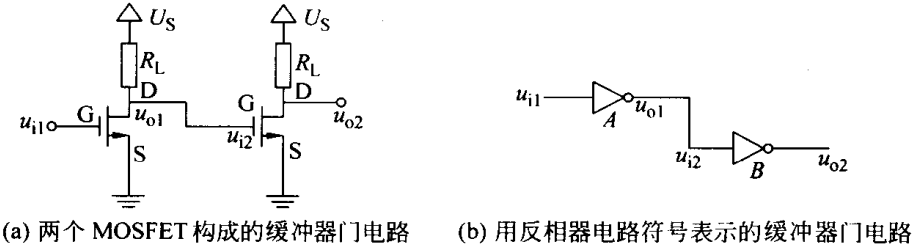
\includegraphics[width=\columnwidth]{assets/反相器的传播延迟.png}
\end{figure}

\subsection{二阶动态电路}

\begin{figure}[H]\centering
    \includegraphics[width=0.8\columnwidth]{assets/RLC.pdf}
    \caption{$RCL$ 电路,左串右并}
\end{figure}

\begin{equation}
y'' + 2\beta y' + \omega_0 y = 0
\end{equation}
经典法:$y_s$ 是稳态解、${\color{red} \omega = \sqrt{|\omega_0^2 - \beta^2|}}$
\begin{gather}
    \begin{aligned}
        &\text{欠阻尼:} \beta < \omega_0, y(t) = y_s +  e^{-\beta t} A\sin \left( \omega t + \phi \right) \\ 
        &     
        \begin{cases}
        y_s = 0 \Longrightarrow 
        t = \frac{\omega}{\beta + \frac{y'(0)}{y(0)}} \ {\color{red} (\text{可负})},\quad A = y(0)\cdot \frac{\sqrt{1 + t^2}}{t},\quad \phi = \arctan t 
        \\
        y_0 = y_s = 0 \Longrightarrow
        A = \frac{y'(0)}{\omega},\quad \phi = 0
        \end{cases}
        \\ 
        &\text{临界阻尼:} \beta = \omega_0, y(t) = y_s +  e^{-\beta t} (A + Bt) \\ 
        &
        \begin{cases}
            A = y(0) - y_s \\
            B = \beta y(0) + y'(0) - \beta y_s
        \end{cases} \\
        &\text{过阻尼:} \beta > \omega_0, y(t) = y_s +  e^{-\beta t}\left( A\,e^{\omega t} + B\,e^{-\omega t}\right) \\ 
        &
        \begin{cases}
            A = \frac{1}{2 \omega} \left[ y'(0) + (\beta + \omega)(y_0 - y_s) \right] \\ 
            B = - \frac{1}{2 \omega} \left[ y'(0) + (\beta - \omega)(y_0 - y_s) \right]
        \end{cases}
    \end{aligned}
\end{gather}
具体电路中,$f$ 可以是 $u_C$ 或 $i_L$ :
\begin{gather}
\text{串联 $RLC$: \ } 
LC f'' + RC f'' + f = h(t) \\ 
\text{并联 $RLC$: \ }
f'' + \frac{f'}{RC} + \frac{f}{LC} = h(t)
\end{gather}

\subsection{冲激响应和阶跃响应}
\begin{gather}
    \delta_0 = \frac{\mathrm{d} \eta_0 }{\mathrm{d} t } ,\quad 
    \text{冲激响应}\  h(t) = \frac{\mathrm{d} s(t)}{\mathrm{d} t},\quad s(t) \text{\ 为阶跃响应}
\end{gather}
注意冲激 $\delta_0$ 前的系数是多少,响应的 $\eta_0$ 也要乘上这个系数。{\color{red} 单位冲激 $U_s = \delta_0$ 下的响应}为:
\begin{table}[H]\centering
\resizebox{\columnwidth}{!}{
    \begin{tabular}{|c|c|c|c|c|c|c|c|c|c|}\hline
        类型 & $RC$ 串 & $RC$ 并 & $RL$ 串 & $RL$ 并  \\
        \hline
        突变 & $\Delta u_C = 1/RC$ & $\Delta u_C = 1/C$ & $\Delta i_L=  1/L$ & $\Delta i_L = R/L$  \\
        \hline
    \end{tabular}
}
\end{table}
任意激励的瞬态响应,先求出单位冲激响应 $h(t)$,则激励 $e$ 下的 {\color{red} 零状态} 响应 $H$ 为:
\begin{equation}
H(t) = e(t) * h(t) = \int_{-\infty}^{+\infty} e(\tau)h(t - \tau) \mathrm{d} \tau
\end{equation}


\section{第六章:正弦激励下电路的稳态分析}

\subsection{功率}

功率:
\begin{gather}
\text{瞬时 (W) : \ } p(t) = u(t) \cdot i(t) \\
\text{有功 (W) : \ } P = UI \cos \varphi = I^2 \Re \{Z\} \\ 
\text{无功 (var) : \ } Q = UI \sin \varphi = I^2 \Im \{Z\} \\
\text{视在 (V$\cdot$A) : \ } S = UI = I^2 |Z| = \sqrt{P^2 + Q^2} \\ 
\text{复功率 (V$\cdot$A) : \ } \dot{S} = P + jQ = \dot{U}\dot{I}^*\\
\text{功率因数 : \ } \cos \varphi = \frac{\Re \{Z\}}{|Z|} = \frac{P}{\sqrt{P^2 + Q^2}} 
\end{gather}

保持有功功率 $P$ 不变,将阻抗角从 $\varphi_1$ 改变到 $\varphi_2$ (仅影响无功功率 $Q$),需要并联的电抗 $j X$ 为:
\begin{equation}
X = \frac{U^2}{P \left(\tan \varphi_2 - \tan \varphi_1\right)}
\end{equation}
特别地:
\begin{gather}
    \text{感性:} \varphi > 0 ,\quad 
    C = \frac{P \left(\tan \varphi_1 - \tan \varphi_2\right)}{\omega U^2}
    \\ 
    \text{容性:} \varphi < 0 , \quad 
    L = \frac{U^2}{\omega P \left(\tan \varphi_2 - \tan \varphi_1\right)}
\end{gather}


\subsection{最大功率传输}
考虑实际电源 ($\dot{U_s}$, $Z_s = R_s + j X_s$) 接在负载 $Z = R + jX$ 两端,则有功功率为:
\begin{equation}
P = \frac{R}{(R + R_s)^2 + (X + X_s)^2} \cdot U_s^2 
\end{equation}
为使负载获得最大有功功率 $P$,有以下几种情况:
\vspace*{-3mm}
\begin{table}[H]\centering
    \renewcommand{\arraystretch}{3} % 调整行间距为 1.5 倍
\resizebox{\columnwidth}{!}{
    \begin{tabular}{cccccccccc}\toprule
        情况 & 满足条件 & 最大功率 $P_{\max}$  \\
        \midrule
        改变 $X$ & $X = -X_s$ & $\displaystyle \frac{R}{(R+R_s)^2} U_s^2$  \\
        改变 $R$ & $R = \sqrt{R_s^2 + (X + X_s)^2}$ & $\displaystyle \frac{1}{2(R_s + R)} U_s^2$  \\
        改变 $X$ 和 $R$ & $Z = Z_s^*$ & $\displaystyle \frac{1}{4R_s} U_s^2$  \\
        $\arg Z = \varphi_s$ 不变,$| Z |$ 可变 & $| Z | = | Z_s |$ & $\displaystyle \frac{\cos \varphi_s}{2 | Z_s | \left[ 1 - \cos (\varphi_s \varphi) \right]}$   \\
        \bottomrule
    \end{tabular}
}
\end{table}



\subsection{频率响应}

常见一阶滤波器的网络函数 $H$、相频特性 $\varphi(\omega)$ 与截止频率 $\omega_c$ 为:
\begin{align*}
\begin{aligned}
&RC \text{低通}, H = \frac{1}{1 + j \omega CR}, 
\varphi = - \arctan \left(\frac{\omega}{\omega_c}\right) &&, \omega_c = \frac{1}{\tau} = \frac{1}{RC}\\
&RC \text{高通}, H = \frac{j \omega CR}{1 + j \omega CR}, 
\varphi = 90^\circ - \arctan \left(\frac{\omega}{\omega_c}\right) &&, \omega_c = \frac{1}{\tau} = \frac{1}{RC}\\
&RL \text{低通}, H = \frac{1}{1 + j \omega \frac{R}{L}}, 
\varphi = - \arctan \left(\frac{\omega}{\omega_c}\right) &&, \omega_c = \frac{1}{\tau} = \frac{R}{L}\\
&RL \text{高通}, H = \frac{j \omega \frac{R}{L}}{1 + j \omega \frac{R}{L}}, 
\varphi = 90^\circ - \arctan \left(\frac{\omega}{\omega_c}\right) &&, \omega_c = \frac{1}{\tau} = \frac{R}{L}
\end{aligned}
\end{align*}

$RC$ 带通滤波器(经缓冲器隔离)的谐振频率 $\omega_0$ 与最大增益 $H_{\max}$ : 
\begin{equation}
\omega_0 = \frac{1}{\sqrt{\tau_1 \tau_2}},\quad 
H_{\max} = \frac{\tau_2}{\tau_1 + \tau_2}
\end{equation}

\subsection{波特图}
求出 $H$ 的表达式,分子为零则零点,分母为零则极点。在画波特图之前,需要先确定 $\lim_{\omega \to 0, \infty} \arg H$ 和  $\lim_{\omega \to 0, \infty} |H|$。然后:
\begin{align}
&\text{$|H|$: 初始斜率为 0,遇到零点斜率增加 20 dB/dec ,遇到极点斜率增加 - 20 dB/dec ;} \\ 
& \text{$\arg H$ : 不受零点影响,经过极点时会有  $0 \to  -45^\circ \to -90^\circ$ 的相位下降。}
\end{align}

\subsection{谐振电路:}

$|Z|$ 极小为串联谐振,$|Z|$ 极大为并联谐振。$RLC$ 串联电路发生谐振时,具有如下特点:
\begin{enumerate}
\item $\dot{U}_S$ 和 $\dot{I}$ 同相,入端阻抗 $Z$ 表现为纯电阻,且模长最小;
\item 在 $\dot{U}_S$ 作为激励下,电流 $\dot{I}$ 达到最大值,响应 $\dot{U}_R$ 达到最大值;
\item 电容和电感电压的幅值都是 $U_S$ 的 $Q$ 倍,且相位相反,即 $\dot{U}_L = -\dot{U}_C = j Q \dot{U}_S$,$Q = \frac{\omega_0 L}{R} = \frac{1}{\omega_0 CR} = \frac{1}{R}\sqrt{\frac{L}{C}}$ 为品质因数;
\item 电源无功功率为 0,只发出有功功率,且完全被电阻消耗;电感与电容之间进行能量交换,与电源没有能量交换。
\end{enumerate}


\noindent $RLC$ 并联电路发生谐振时,具有如下特点:
\begin{enumerate}
\item $\dot{U}$ 和 $\dot{I}_S$ 同相,入端导纳 $Y$ 表现为纯电导,且模长最小;
\item 在 $\dot{I}_S$ 作为激励下,电压 $\dot{U}$ 达到最大值,响应 $\dot{U}_R$ 达到最大值;
\item 电容和电感电流的幅值都是 $I_S$ 的 $Q$ 倍,且相位相反,即 $\dot{I}_L = -\dot{I}_C = jQ \dot{I}_S$,$Q = \omega_0 C R = \frac{R}{\omega_0 L} = R\sqrt{\frac{C}{L}}$ 品质因数;
\item 电源无功功率为 0,只发出有功功率,且完全被电阻消耗;电感与电容之间进行能量交换,与电源没有能量交换。
\end{enumerate}

\subsection{品质因数}
\begin{gather}
RLC \text{\ 串联:} Q = \frac{\omega_0 L}{R} = \frac{\rho}{R} = \frac{1}{\omega_0 CR} = \frac{1}{R}\sqrt{\frac{L}{C}} \\ 
RLC \text{\ 并联:} Q = \frac{R}{\omega_0 L} = \omega_0 C R =  R\sqrt{\frac{C}{L}}
\end{gather}
其中$\rho = \omega_0 L$ 是特性阻抗。$RLC$ 串并联电路归一化频响:
\begin{equation}
I_\text{norm} = \frac{I(\eta \, \omega_0)}{I(\omega_0)} = \frac{1}{\sqrt{ 1 + Q^2 \left(\eta - \frac{1}{\eta}\right)^2 }},\quad \eta = \frac{\omega}{\omega_0}
\end{equation}
\begin{equation}
\text{WB} = \frac{\omega_0}{Q},\quad \text{$Q$ 是谐振电路的品质因数}
\end{equation}
电感和电容的品质因数:
\begin{equation}
Q_L = \frac{\omega L}{R\text{dcr}},\quad 
Q_C = \frac{1}{\omega C R_{\text{esr}}}
\end{equation}

$Q$ 的三种物理意义角度:
\begin{gather}
\begin{cases}
    \text{电压电流 amptitude 角度:} \text{串联\ } U_L = U_C = Q U_S,\
    \text{并联\ } I_L = I_C = Q I_S \\
    \text{能量角度:} \text{$Q$ 大时,存储能量多,损耗能量小} \\
    \text{频率响应角度: 归一化频响曲线} 
\end{cases}
\end{gather}

\subsection{互感}

无论同名端、电流电压参考方向如何,我们有以下结论:
\begin{enumerate}
\item 电流流入同名端,则为正,流出则为负;
\item 电压正端在同名端,则无需取反,反之需取反;
\end{enumerate}
上面的结论对多个线圈的互感也适用。

\begin{figure}[H]\centering
    \includegraphics[width=0.8\columnwidth]{assets/电感去耦等效.png}
    \caption{电感去耦等效}
    \label{电感去耦等效}
\end{figure}

利用去耦等效计算某电感两端电压,{\color{red} 勿忘电感电压参考端会发生移动}。
\begin{gather}
    \begin{cases}
    \text{同侧串联:} L_{\text{eq}} = L_1 + L_2 + 2M \\
    \text{异侧串联:} L_{\text{eq}} = L_1 + L_2 - 2M
    \end{cases} \\
    \begin{cases}
    \text{同侧并联:} L_{\text{eq}} = M + (L_1 - M)\parallel(L_2 - M)\\
    \text{异侧并联:} L_{\text{eq}} = -M + (L_1 + M)\parallel(L_2 + M)
    \end{cases}
\end{gather}

\subsection{变压器}
非理想变压器等效:
\begin{figure}[H]\centering
    \includegraphics[width=0.8\columnwidth]{assets/非理想变压器 2.pdf}
    \caption{非理想变压器的等效}
    \label{非理想变压器等效}
\end{figure}
\begin{figure}[H]\centering
    \includegraphics[width=0.8\columnwidth]{assets/非理想变压器 (2).pdf}
\end{figure}

\begin{gather}
\text{原边引入阻抗:} \frac{(\omega M)^2}{Z_2} \\
\text{副边引入阻抗:} \frac{(\omega M)^2}{Z_1},\quad 
\text{副边引入电源:} \dot{U}_{\text{eq}} = \frac{j \omega M}{Z_1} \dot{U}_1
\end{gather}

当耦合系数 $k = \frac{M}{\sqrt{L_1 L_2}} = 1$ 时,称为全耦合,此时将变压器看作二端口网络,则有:
\begin{gather}
\begin{cases}
\dot{U}_1 = n \dot{U}_2 \\ 
\dot{I}_1 = \frac{\dot{U}_1}{j \omega L_1} + \frac{1}{n} (- \dot{I}_2)
\end{cases}
,\quad 
\begin{bmatrix}
    \dot{U}_1 \\ \dot{I}_1 
\end{bmatrix}
= 
\begin{bmatrix}
    n & 0 \\ 
    \frac{1}{j \omega L_1} & \frac{1}{n} 
\end{bmatrix}
\begin{bmatrix}
    \dot{U}_2 \\ 
    - \dot{I}_2
\end{bmatrix} \\
\Longrightarrow 
T = 
\begin{bmatrix}
    n & 0 \\ 
    \frac{1}{j \omega L_1} & \frac{1}{n} 
\end{bmatrix}
\end{gather}
上面的变压器称为全耦合变压器,其中 $n \propto \sqrt{\frac{L_1}{L_2}}$。特别地,当 $L_1$ 足够大时,$\frac{\dot{U}_1}{j\omega L_1}$ 一项可以忽略,此时有:
\begin{equation}
    \dot{U}_1 = n \dot{U}_2,\quad \dot{I}_1 =  - \frac{1}{n} \dot{I}_2
\end{equation}
即为喜闻乐见的理想变压器。理想变压器具有负载“放大”功能,设原线圈比幅线圈为 $n$,则在原线圈中有:
\begin{equation}
Z_{\text{eq}} = n^{2} Z
\end{equation}

\subsection{三相电路}

%\begin{figure}[H]\centering
%    \includegraphics[width=0.35\columnwidth]{assets/三相电路/image.png}
%    \caption{三相电路的线序}
%\end{figure}


\begin{gather}
    \text{$\Delta$ 型负载:}
    \begin{cases}
        \dot{I}_A = \sqrt{3} \, \dot{I}_{AB} \angle -30^\circ \\
        \dot{I}_B = \sqrt{3} \, \dot{I}_{BC} \angle -30^\circ \\
        \dot{I}_C = \sqrt{3} \, \dot{I}_{CA} \angle -30^\circ
    \end{cases}
    \\
    \text{Y 型负载:}
    \begin{cases}
        \dot{U}_{AB} = \sqrt{3} \, \dot{U}_{AN} \angle 30^\circ \\
        \dot{U}_{BC} = \sqrt{3} \, \dot{U}_{BN} \angle 30^\circ \\
        \dot{U}_{CA} = \sqrt{3} \, \dot{U}_{CN} \angle 30^\circ
    \end{cases}
\end{gather}

\begin{figure}[H]\centering
\begin{subfigure}[b]{0.5\columnwidth}\centering
    \includegraphics[height=60pt]{assets/三相电路/image copy.png}
    \caption{$\Delta$ 型负载}
\end{subfigure}\hfill
\begin{subfigure}[b]{0.5\columnwidth}\centering
    \includegraphics[height=65pt]{assets/三相电路/image copy 2.png}
    \caption{Y 型负载}
\end{subfigure}
\caption{对称负载三相电路}
\end{figure}

$\Delta$ 型电源和$\Delta$ 型负载变换为 $Y$ 型:
\begin{equation}
\begin{cases}
\dot{U}_{AN} = \frac{1}{\sqrt{3}} \dot{U}_{AB} \angle -30^\circ \\
\dot{U}_{BN} = \frac{1}{\sqrt{3}} \dot{U}_{BC} \angle -30^\circ \\
\dot{U}_{CN} = \frac{1}{\sqrt{3}} \dot{U}_{CA} \angle -30^\circ
\end{cases},\quad 
Z_{Y} = \frac{Z_{\Delta}}{3}
\end{equation}
对称负载 $\dot{U}_{N'N} \equiv 0$,$\dot{I}_{N'N} \equiv 0$,$Z_N$ 对电路没有影响(虚短+虚断)。

\subsection{非对称三相电路}

负载不对称时,需要区分有没有中线。如果存在中线($Z_N = 0$),负载电压仍等于相电压,直接抽单相计算即可;如果不存在中线($Z_N = \infty$),:
\begin{gather}
\dot{U}_{N'N} = \frac{ \frac{\dot{U}_{AN}}{Z_A} + \frac{\dot{U}_{BN}}{Z_B} + \frac{\dot{U}_{CN}}{Z_C}  }{ \frac{1}{Z_A} + \frac{1}{Z_B} + \frac{1}{Z_C} } \\
\dot{I}_{A} = \frac{\dot{U}_{AN} - \dot{U}_{N'N} }{Z_A}, \quad 
\dot{I}_{B} = \frac{\dot{U}_{BN} - \dot{U}_{N'N} }{Z_B}
\end{gather}

\subsection{三相电路的功率}

将相电压、相电流的下标用 p 表示 (phase),将线电压、线电流的下标用 l 表示 (line),则对称三相电路的各功率为:
\begin{equation}
P = 3 U_p I_p \cos \varphi,\quad 
Q = 3 U_p I_p \sin \varphi,\quad
S = 3 U_p I_p
\hat{S} = 3 \dot{U}_p \dot{I}_p^*
\end{equation}
可以推出,对称三相电路的瞬时功率 $p \equiv 3 U_p I_p \cos \varphi = P$。两表法测三相电路功率的示意图如下:
\begin{figure}[H]\centering
    \includegraphics[width=\columnwidth]{assets/三相电路/image copy 5.png}
    \caption{两表法测三相电路功率}
\end{figure}

以共 C 接法为例,两表的功率示数为:
\begin{gather}
P_1 = U_{AC} I_A \cos (\varphi_{u_{AC}} - \varphi_{i_A})\\
P_2 = U_{BC} I_B \cos (\varphi_{u_{BC}} - \varphi_{i_B})
\end{gather}
设 $Y$ 型电源下的 $\dot{U}_A$,$\dot{I}_A$ 已知,则 $\dot{U_{AB}} = \sqrt{3} U_A \angle 30^\circ$,设功率因数为 $\varphi$,则两表读数为:
\begin{gather}
P_1 = \sqrt{3} U_A I_A \cos (\varphi - 30^\circ)
P_1 = \sqrt{3} U_A I_A \cos (\varphi + 30^\circ)
\end{gather}

用单个功率表测对称电路的无功功率:
\begin{figure}[H]\centering
    \includegraphics[width=0.4\columnwidth]{assets/QQ_1735491515790.png}
\end{figure}
\begin{figure}[H]\centering
    \includegraphics[width=0.4\columnwidth]{assets/image copy 3.png}
\end{figure}





\subsection{提高功率因数}

为提高功率因数,同时考虑到安全性,通常对感性电路($\varphi > 0$,电压带动电流)并联 Y 型电容组,对容性电路($\varphi < 0$,电流带动电压)并联 Y 型电感组。并联电容时计算公式如下:
\begin{equation}
\varphi > 0,\quad \text{感性:}
C = \frac{P(\tan \varphi_1 - \tan \varphi_2)}{3\,\omega U^2}
\end{equation}
如果上式计算出 $C < 0$,则需要并联电感,计算公式为:
\begin{equation}
\varphi < 0,\quad \text{容性:}
L = \frac{3 U^2}{\omega \, P (\tan \varphi_2 - \tan \varphi_1)}
\end{equation}
等价地讲,为了将一个 $\varphi_1$ 变换到 $\varphi_2$,需要并联的电抗 $X$ 为:
\begin{equation}
X = \frac{3 U^2}{P (\tan \varphi_2 - \tan \varphi_1)},\quad 
Z = j X = j \frac{3 U^2}{P (\tan \varphi_2 - \tan \varphi_1)} 
\end{equation}

也可以考虑并联 $\Delta$ 型电容,但 Y 型时电容承受相电压,$\Delta$ 型承受线电压(通常更大),后者耐压要求更高。


\subsection{周期性非正弦激励的电路稳态分析}

通常是计算非正弦激励下的电压、电流或功率,只需分解为多个频率量,分别计算后利用叠加定理相加即可。注意不同频率下元件的阻抗不同,灵活运用串联、并联谐振以简化分析。功率之所以可以直接相加,是因为其为“不同频率“激励下的功率,而不是早先讨论的纯直流激励下的功率,前者互不影响,后者不能直接相加。需要注意,若已知非正弦激励下的电压有效值和电流有效值,{\color{red} 不能简单的用 $P = U I \cos \varphi$ 来求有功功率 $P$},因为不同频率分量的 $\varphi$ 不同。需要分别计算后将它们相加。{\color{red} 注意变压器在 DC 不起作用}。


\section{其它}

\subsection{$Y$ 型与 $\Delta$ 型电阻}
\begin{gather}
    \begin{matrix}
        \text{由 Y 求 $\Delta$ :}\quad R_{12}= R_1 + R_2 + \frac{R_1R_2}{R_3}, \quad
        R_{13}=R_1 + R_3 + \frac{R_1R_3}{R_2} \\
        \text{由 $\Delta$ 求 Y :}\  R_{1}=\frac{R_{12}R_{13}}{R_0},\ 
        R_{2}=\frac{R_{21}R_{23}}{R_0},\ 
        R_0 = R_{12}+R_{13}+R_{23} 
    \end{matrix}
\end{gather}

\subsection{二端口}
传输矩阵 $\boldsymbol{T}$ :
\begin{gather}
\begin{bmatrix}
    u_1 \\ i_1
\end{bmatrix}
= 
\boldsymbol{T}\cdot
\begin{bmatrix}
    u_2 \\ {\color{red} -i_2}
\end{bmatrix}
,\quad 
\text{互易:} AD - BC = 1,\quad 
\text{对称:} A = D
\end{gather}
二端口吸收的功率:
\begin{equation}
P = u_1 i_1 + u_2 i_2
\end{equation}
若一个二端口网络 N 是对称的,则当 $u_1, i_1, u_2, i_2$ 已知时,其传输矩阵的计算公式如下:
\begin{equation}
\boldsymbol{T} = 
\begin{bmatrix}
    A & B \\ 
    C & D
\end{bmatrix}
=
\begin{bmatrix}
    \frac{i_1}{i_2} & \frac{u_1}{i_2} \\ 
    \frac{AD - 1}{B} & \frac{i_1}{i_2}
\end{bmatrix}
\end{equation}
二端口级联:
\begin{equation}
\boldsymbol{T} = \boldsymbol{T}_1 \cdot \boldsymbol{T}_2
\end{equation}
与电阻级联:
\begin{equation}
T = 
\begin{bmatrix}
    1 & R \\ 
    0 & 1
\end{bmatrix}
\cdot 
\begin{bmatrix}
    A & B \\
    C & D
\end{bmatrix}
= 
\begin{bmatrix}
    A + CR & B + DR \\
    C & D
\end{bmatrix}
\end{equation}

\begin{figure}[H]\centering
\begin{subfigure}[b]{0.55\columnwidth}\centering
    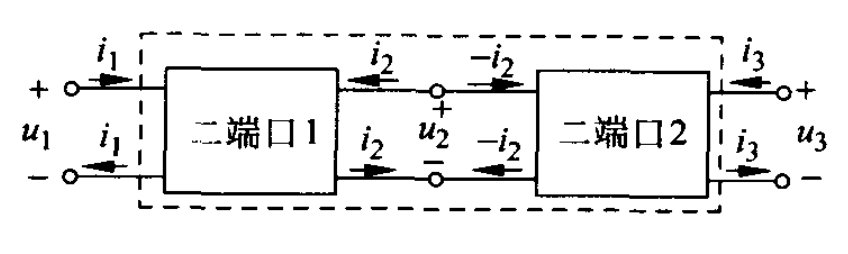
\includegraphics[height=30pt]{assets/级联.png}
\end{subfigure}\hfill
\begin{subfigure}[b]{0.45\columnwidth}\centering
    \includegraphics[height=30pt]{assets/image.png}
\end{subfigure}
\end{figure}

注意如果 $R$ 在右边,乘法顺序相反。

\subsection{杂七杂八}
\begin{enumerate}
    \item 三相电路:三线即为 $\Delta$ 型,需除以 $\sqrt{3}$;
\item 380 V $\overset{\frac{1}{\sqrt{3}}}{\longrightarrow}$ 220 V;
\item 感性 $\varphi = 40^\circ $,$\dot{U} = 220 \angle 0$,则 $\dot{I} = 10 \angle {\color{red} -40^\circ}$;
\item 家用电频率、工频 50 Hz;
\item {\color{red} 注意变压器在 DC 不起作用};
\item 相电压相电流:

\begin{gather}
\text{线电压:} \dot{U}_{AB}, \quad \text{线电流:} \dot{I}_A \\
\text{相电压:} \dot{U}_A, \quad \text{相电流:} \dot{I}_{AB}
\end{gather}
\begin{figure}[H]\centering
\begin{subfigure}[b]{0.5\columnwidth}\centering
    \includegraphics[height=85pt]{assets/相电压线电压电流 - 副本 (2).pdf}
\end{subfigure}\hfill
\begin{subfigure}[b]{0.5\columnwidth}\centering
    \includegraphics[height=85pt]{assets/相电压线电压电流 - 副本.pdf}
\end{subfigure}
\end{figure}

\item 三相电路的戴维南等效,先求开路电压 $U_{\text{oc}}$,然后置零,求端口电阻:
\begin{equation}
Z_{\text{eq}} = 2 \left( Z_1 \parallel Z_2 \right) = 2 \left( r \parallel Z \right)
\end{equation}
\begin{figure}[H]\centering
    \includegraphics[width=0.6\columnwidth]{assets/image copy.png}
\end{figure}
\begin{figure}[H]\centering
    \includegraphics[width=0.6\columnwidth]{assets/image copy 2.png}
\end{figure}

\item $RC$ 低通滤波器的波特图:
\begin{figure}[H]\centering
    \includegraphics[width=0.80\columnwidth]{assets/波特图/RC 低通 波特图.pdf}
\end{figure} 

\item 全通滤波器(移相桥):

全通滤波器是一种比较特殊的滤波器,具有平坦的幅频特性,主要用来产生相移,例如下面的移相桥:
\begin{gather}
H(\omega) = \frac{1}{2}\cdot\frac{j\omega R_0C - 1}{j\omega R_0C + 1},\quad \theta = 180^{\circ} - 2 \arctan \left(\frac{\omega}{\omega_c} \right)\\
\omega_c = R_0C
\end{gather}

%\begin{figure}[H]\centering
%\begin{subfigure}[b]{\columnwidth}\centering
%    \includegraphics[height=45pt]{assets/移相桥.png}
%    \caption{移相桥电路图}
%\end{subfigure}\hfill
%\begin{subfigure}[b]{\columnwidth}\centering
%    \includegraphics[height=45pt]{assets/移相桥幅频.png}
%    \caption{幅频特性}
%\end{subfigure}
%\begin{subfigure}[b]{\columnwidth}\centering
%    \includegraphics[height=45pt]{assets/移相桥相频.png}
%    \caption{相频特性}
%\end{subfigure}
%\caption{全通滤波器移相桥}
%\end{figure}

\item dB 单位转换:
\begin{table}[H]\centering
    %\renewcommand{\arraystretch}{1.5} % 调整行间距为 1.5 倍
    %\setlength{\tabcolsep}{1.5mm} % 调整列间距
    \caption{增益与 dB 值的对应关系}
    \label{增益与 dB 值的对应关系}
\resizebox{\columnwidth}{!}{
    \begin{tabular}{cccccccccc}\toprule
        $H$ & 0.01 & 0.1 & 0.5 & $\frac{1}{\sqrt{2}}$ & \textbf{1} & $\sqrt{2}$ & 2 & 10 & 100 \\
        \midrule
        $H_{\text{dB}}$ & -40 & -20 & -6 & -3 & \textbf{0} & 3 & 6 & 20 & 40 \\
        \bottomrule
    \end{tabular}
}
\end{table}

\item 识别变压器同名端:
\begin{figure}[H]\centering
    \includegraphics[width=0.85\columnwidth]{assets/0a2707b2610d952a8f63f9bcfc51616f.png}
\end{figure}

\begin{figure}[H]\centering
    \includegraphics[height=\columnwidth, angle=-90]{assets/扫描全能王 2024-12-30 21.25.pdf}
\end{figure}

\end{enumerate}
% --------------------------------------------------------- %
% --------------------------------------------------------- %
\end{multicols*}  
\end{document}
% --------------------------------------------------------- %
% --------------------------------------------------------- %